\documentclass[10pt, compress]{beamer}
% Modern, fancy theme with great contrast
\usetheme{Madrid}
\usecolortheme{whale}
\useoutertheme{shadow}
\usepackage{amsmath,amssymb,amsthm}
\usepackage{graphicx}
\usepackage{hyperref}
\usepackage{booktabs}
\usepackage{array}
\newtheorem{proposition}{Proposition}
% Define block colors for stylistic effects
\setbeamercolor{block title}{bg=blue!80!black, fg=white}
\setbeamercolor{block body}{bg=blue!10, fg=black}
\setbeamercolor{block title example}{bg=green!60!black, fg=white}
\setbeamercolor{block body example}{bg=green!10, fg=black}
\setbeamercolor{block title alerted}{bg=red!70!black, fg=white}
\setbeamercolor{block body alerted}{bg=red!10, fg=black}
\title[CS648: Primality Testing]{Primality Testing:\\Theory, Implementation, and Experimental Comparison}
\subtitle{An Advanced Dive into Miller-Rabin, Arbitrary Precision, and Benchmarks}
\author[Group 230272]{Group No. 230272}
\institute[CS648]{CS648 Project Presentation}
\date{\today}
\begin{document}
\begin{frame}
    \titlepage
\end{frame}
\begin{frame}{Table of Contents}
    \tableofcontents[hideallsubsections]
\end{frame}
% ----------------------------------------------------------------------
\section{1. The Motivation \& Problem Statement}
% ----------------------------------------------------------------------
\begin{frame}{The Primality Problem}
    \textbf{Primality testing} asks a deceptively simple question: Is a given positive integer $n$ prime or composite?
    
    \pause
    \vspace{0.3cm}
    Why do we need computationally fast testing?
    \begin{itemize}
        \item<3-> \textbf{Public-Key Cryptography (RSA):} Requires the generation of extremely large prime keys (e.g., 2048 to 4096 bits).
        \item<4-> \textbf{Generating Primes:} Generating a prime practically means generating random odd numbers and testing them until one passes.
        \item<5-> \textbf{The Catch:} Standard exact factoring tests scale exponentially. Trying to divide a 4096-bit number by all odd integers up to its square root would take longer than the lifespan of the universe.
    \end{itemize}
    
    \onslide<6->
    \begin{alertblock}{The Engineering Dilemma}
    We cannot afford mathematically "perfect but slow" deterministic tests. We need an algorithm resolving 4096-bit computations in milliseconds.
    \end{alertblock}
\end{frame}
\begin{frame}{Baseline Alternatives}
    Before covering the optimal solution, let's look at the benchmarks.
    
    \pause
    \begin{block}{The Square-Root Method}
        \begin{itemize}
            \item Tests divisibility by integers up to $\sqrt{n}$.
            \item Exact, but strictly limited by an $\mathcal{O}(\sqrt{n})$ runtime. Hits a wall around $50$ bits.
        \end{itemize}
    \end{block}
    
    \pause
    \begin{block}{The AKS Primality Test}
        \begin{itemize}
            \item Revolutionized theory by proving \textbf{PRIMES $\in$ P}.
            \item Deterministic polynomial time. 
            \item However, the overhead constant is gigantic. In our implementation, testing a 60-bit prime with AKS already stalls execution significantly.
            \item The AKS code in this project was written by ChatGPT.
        \end{itemize}
    \end{block}

    \vspace{0.2cm}
    {\tiny Reference: M. Agrawal, N. Kayal, and N. Saxena, \textit{PRIMES is in P}, Annals of Mathematics, 160(2), 781--793, 2004.}
\end{frame}
% ----------------------------------------------------------------------
\section{2. Mathematical Build-up (The Proofs)}
% ----------------------------------------------------------------------
\begin{frame}{Fermat's Little Theorem}
    The classical starting point for primality testing is Fermat's Little Theorem.
    
    \pause
    \begin{theorem}
    If $p$ is prime and $\gcd(a, p) = 1$, then:
    \[ a^{p-1} \equiv 1 \pmod{p} \]
    \end{theorem}
    
    \pause
    \begin{alertblock}{The Carmichael Trap (The Weakness)}
    Unfortunately, reversing the theorem is imperfect. There are composite numbers $n$ that satisfy $a^{n-1} \equiv 1 \pmod{n}$ for \textit{all} bases $a$ coprime to $n$. \\
    These are called \textbf{Carmichael numbers} (e.g., $561 = 3 \times 11 \times 17$).
    \end{alertblock}
\end{frame}
\begin{frame}{Fermat Experiments on Composite Numbers}
    \begin{columns}[T]
        \column{0.5\textwidth}
        \centering
        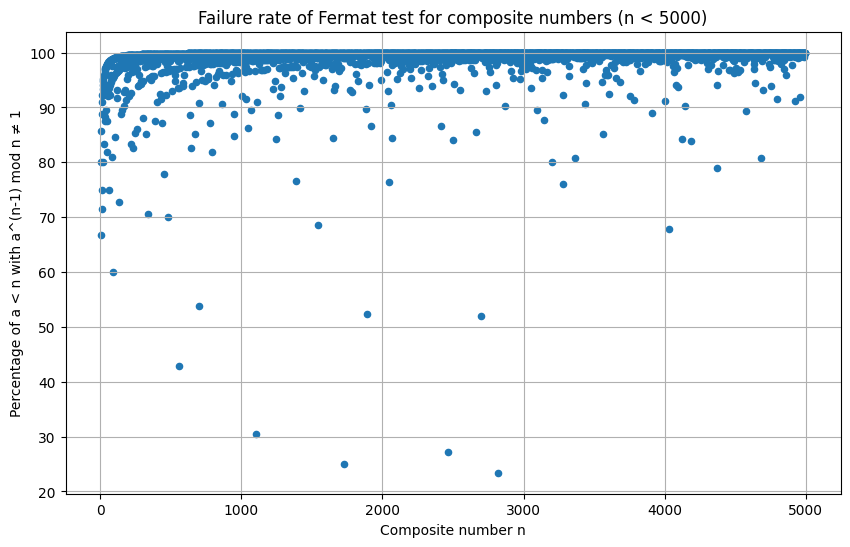
\includegraphics[width=0.95\textwidth,height=0.58\textheight,keepaspectratio]{experiment_plots/failure_fermat.png}
        
        {\footnotesize All bases $a<n$: most composite numbers fail Fermat for a large fraction of bases.}
        
        \column{0.5\textwidth}
        \centering
        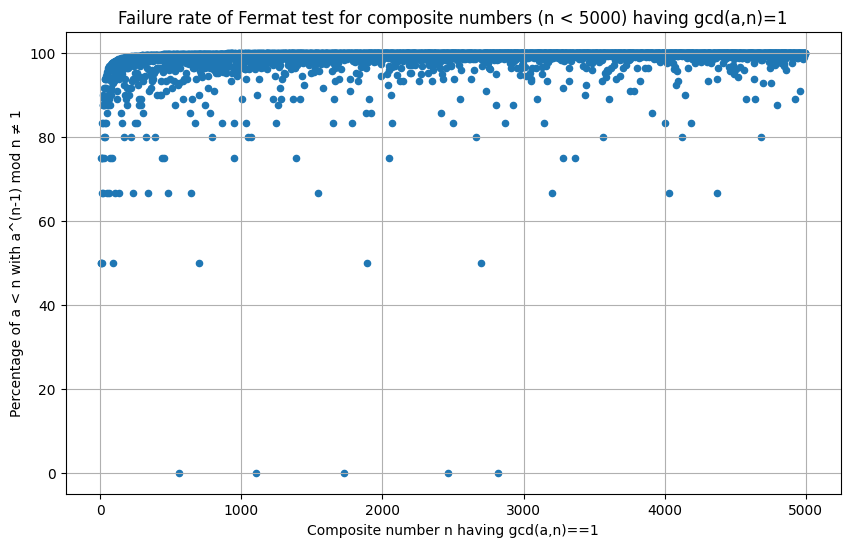
\includegraphics[width=0.95\textwidth,height=0.58\textheight,keepaspectratio]{experiment_plots/failure_fermat_among_gcd(a,n)_1.png}
        
        {\footnotesize Only coprime bases: Carmichael numbers appear as low-failure outliers.}
    \end{columns}
    
    \vspace{0.2cm}
    \textbf{Key observation:} For non-Carmichael composites, the coprime-base failure rate stays at or above $50\%$, which matches the half-witness result used to motivate a stronger test.
\end{frame}
\begin{frame}{Building a Stronger Test: Step 1 (GCD Failures)}
    \textbf{Question:} Which bases $a$ can trick the Fermat test when $n$ is composite?
    
    \pause
    \begin{lemma}
    If $1 < a < n$ and $\gcd(a, n) > 1$, then $a^{n-1} \not\equiv 1 \pmod{n}$.
    \end{lemma}
    
    \pause
    \begin{proof}
        \begin{itemize}[<+->]
            \item Let $g = \gcd(a, n) > 1$.
            \item Assume for contradiction $a^{n-1} \equiv 1 \pmod{n}$. This implies $n \mid (a^{n-1} - 1)$.
            \item Since $g \mid n$, we have $g \mid (a^{n-1} - 1)$.
            \item Since $g \mid a$, we have $g \mid a^{n-1}$.
            \item Thus $g$ divides their difference: $a^{n-1} - (a^{n-1} - 1) = 1$.
            \item A contradiction, as no $g > 1$ can divide 1.
        \end{itemize}
    \end{proof}
    
    \onslide<8->
    \textit{Conclusion:} Only bases coprime to $n$ can possibly fool Fermat.
\end{frame}
\begin{frame}{Building a Stronger Test: Step 2 (Mappings)}
    To establish probability bounds, we look at mappings over the group.
    
    \pause
    \begin{lemma}
    Let $a$ and $p$ be coprime. For integers $1 \le i, j < p$ and $i \ne j$, we have:
    \[ (a \cdot i) \bmod p \ne (a \cdot j) \bmod p \]
    \end{lemma}
    
    \pause
    \begin{proof}
        \begin{itemize}[<+->]
            \item Assume $(a \cdot i) \bmod p = (a \cdot j) \bmod p$.
            \item Then $a \cdot (i - j) \equiv 0 \pmod p$.
            \item Since $\gcd(a, p) = 1$, by B\'{e}zout's identity $ax + py = 1$.
            \item Multiplying both sides by $x$ implies that $(i - j) \equiv 0 \pmod p$.
            \item Since $1 \le i, j < p$, this contradicts $i \ne j$.
        \end{itemize}
    \end{proof}
    
    \onslide<7->
    \textit{Conclusion:} Modular multiplication by a coprime element acts as a pure bijection.
\end{frame}
\begin{frame}{Building a Stronger Test: Step 3 (Half Witnesses)}
    \begin{proposition}
    If there is \textbf{at least one} coprime witness $x_j$ that fails Fermat's check modulo $a$, then \textbf{at least half} of all coprime elements fail it.
    \end{proposition}
    
    \pause
    \begin{proof}[Proof Sketch]
        \begin{itemize}[<+->]
            \item Let $S$ be the set of elements coprime to $a$. Assume exactly one $x_j \in S$ is a witness: $x_j^{a-1} \not\equiv 1 \pmod a$.
            \item Suppose for contradiction more than half the elements in $S$ are "liars" (they evaluate to $1$). Call this set $S'$.
            \item Construct $S'' = \{(x_j \cdot x_i) \bmod a \mid x_i \in S'\}$.
            \item Every element in $S''$ gives: $(x_j \cdot x_i)^{a-1} \equiv x_j^{a-1} \cdot 1 \not\equiv 1 \pmod a$.
            \item Thus, $S''$ is a set of witnesses exactly the same size as $S'$.
            \item This forces $|S| = |S'| + |S''| > |S|$, a mathematical impossibility.
        \end{itemize}
    \end{proof}
\end{frame}
% ----------------------------------------------------------------------
\section{3. The Miller-Rabin Test}
% ----------------------------------------------------------------------
\begin{frame}{The Miller-Rabin Approach}
    Miller-Rabin circumvents Carmichael numbers by tracking the \textbf{root sequence} leading to 1.
    
    \pause
    \textbf{1. Factor Out Powers of 2}
    For an odd integer $n > 2$, write:
    \[ n - 1 = 2^s d \quad (\text{where } d \text{ is odd}) \]
    
    \pause
    \textbf{2. Squaring Sequence}
    For a chosen base $a$, define:
    \[ x_0 = a^d \pmod n \]
    \[ x_1 = x_0^2, \ x_2 = x_1^2, \dots, \ x_s = x_{s-1}^2 \pmod n \]
    
    \pause
    \textbf{3. Acceptance Rule}
    If $n$ is prime, the sequence must either:
    \begin{itemize}
        \item Start as $1$ ($x_0 \equiv 1 \pmod n$)
        \item Encounter $-1$ right before it hits $1$ ($x_r \equiv -1 \pmod n$)
    \end{itemize}
\end{frame}
\begin{frame}{Why Do Primes Never Fail?}
    \begin{lemma}
    If $p$ is an odd prime, and $x^2 \equiv 1 \pmod p$, then $x \equiv \pm 1 \pmod p$.
    \end{lemma}
    
    \pause
    \begin{proof}
        $x^2 - 1 \equiv 0 \implies (x-1)(x+1) \equiv 0 \pmod p$. Since $p$ is prime, $\mathbb{Z}/p\mathbb{Z}$ has no zero divisors, so $x \equiv 1$ or $x \equiv -1$.
    \end{proof}
    
    \pause
    \begin{theorem}
    If $n$ is an odd prime, the Miller-Rabin test never falsely rejects it.
    \end{theorem}
    \pause
    \begin{proof}[Proof Summary]
        Fermat dictates the sequence ends at $1$ ($x_s = 1$). If $x_0 \not\equiv 1$, there must be a \textbf{first} index $j$ where $x_j \equiv 1$. Therefore, $x_{j-1}^2 \equiv 1$. By the lemma, $x_{j-1}$ must be $-1$. Thus, the sequence perfectly satisfies the Miller-Rabin accept condition.
    \end{proof}
\end{frame}
% ----------------------------------------------------------------------
\section{4. Error Bounds for Composites}
% ----------------------------------------------------------------------
\begin{frame}{Bounding the Strong Liars}
    Composite integers that manage to pass the test are called \textbf{strong liars}. How small is this set probabilistically?
    
    \pause
    \textbf{The Group Theoretic Verification:}
    We do not present the proof in this talk. We only use the final group-theoretic result for Miller-Rabin.
    
    \pause
    \begin{itemize}
        \item For any odd composite number $n$, the bases that falsely make Miller-Rabin accept are only a limited fraction of all valid bases.
        \item The final bound is that at most one fourth of the possible bases are strong liars.
    \end{itemize}
    
    \pause
    \begin{block}{Final Result}
    If $n$ is an odd composite, the set of strong liars satisfies:
    \[ |L(n)| \le \frac{\varphi(n)}{4} \]
    \end{block}
\end{frame}
\begin{frame}{Probabilistic Absolute Certainty}
    Because $|L(n)| \le \frac{\varphi(n)}{4}$:
    \pause
    \begin{itemize}
        \item For an odd composite, a random base $a$ passes with a highest probability of $\frac{1}{4}$.
        \item By testing $k$ independent bases, the probability of false acceptance becomes $\le (\frac{1}{4})^k$.
    \end{itemize}
    
    \pause
    \begin{exampleblock}{Practical Implementation}
    If $k = 40$ random bases are tested independently, the chance of a composite slipping through is $\le 4^{-40} \approx 8.27 \times 10^{-25}$. It is computationally flawless for any realistic threshold.
    \end{exampleblock}
\end{frame}
% ----------------------------------------------------------------------
\section{5. Software Engineering and Implementation Architecture}
% ----------------------------------------------------------------------
\begin{frame}{C++ Implementation Workflow}
    Theory dictates functionality, but engineering provides execution.
    
    \pause
    \begin{block}{1. The \texttt{big\_int} Class Context}
        \begin{itemize}
            \item Normal 64-bit integer registers overflow instantly for cryptographic parameters.
            \item Our custom C++ class stores numbers in arrays mapped in $10^9$ block intervals.
            \item Overlaods logic for addition, subtraction, arithmetic shifting, and most crucially, modular division.
        \end{itemize}
    \end{block}
    
    \pause
    \begin{block}{2. Specialized \texttt{fast\_mod}}
        \begin{itemize}
            \item In $a^b \pmod n$, repeated squaring causes enormous overhead.
            \item We implemented a dedicated \texttt{fast\_mod} that isolates remainder operations strictly without executing a full arbitrary-scale division stack.
        \end{itemize}
    \end{block}
\end{frame}
\begin{frame}{Algorithm Pipeline: \texttt{miller\_rabin.cpp}}
    We structure our test using a fixed witness array to allow deterministic reproducibility up to the native threshold before scaling constraints apply.
    
    \pause
    \begin{itemize}
        \item \textbf{Witness Set:} Fixed array $\{2, 3, 5, 7, 11, 13, 17, 19, 23\}$.
        \item \textbf{Prime Search Workflow:}
            \begin{enumerate}
                \item Randomize bits between structural limits.
                \item Impose odd sizing by clamping LSB.
                \item \textit{Pre-filtering:} Divide quickly by $2, 3, 5, \dots$ to filter out 90\% of candidates cleanly.
                \item Pipe surviving candidates into full Miller-Rabin suite.
            \end{enumerate}
    \end{itemize}
    
    \pause
    We also implemented sequential neighbor search targets, allowing the workflow to hunt for the \texttt{Next\_Prime} and \texttt{Prev\_Prime} off arbitrary starting data.
\end{frame}
\begin{frame}{Interface and Visualization}
    The project encompasses fully featured endpoints so the C++ arithmetic isn't stranded.
    
    \pause
    \begin{block}{CLI Automation (\texttt{primality\_backend.exe})}
        \begin{itemize}
            \item Takes parsed inputs and operates the C++ heavy-lifting behind the scenes.
            \item Output is strictly structured (Key-Value) to pipe into our benchmarking telemetry.
        \end{itemize}
    \end{block}
    
    \pause
    \begin{block}{GUI Interface (\texttt{primality\_gui.py})}
        \begin{itemize}
            \item Full Tkinter interface wrapper allowing humans to input decimal \& hexadecimal arrays, triggering background validations transparently.
            \item The same interface also exposes prime generation and neighbor-prime discovery, making the implementation demonstrable without touching the command line.
        \end{itemize}
    \end{block}
\end{frame}
\begin{frame}{GUI Demonstration}
    \begin{columns}[T]
        \column{0.5\textwidth}
        \centering
        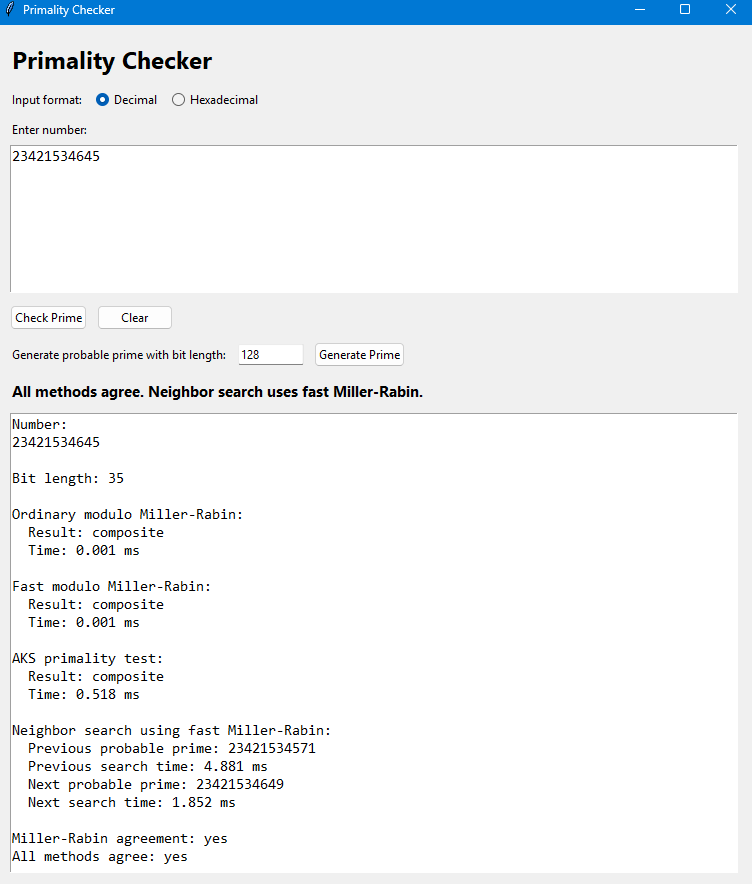
\includegraphics[width=0.92\textwidth,height=0.68\textheight,keepaspectratio]{gui_pictures/gui_check_prime.png}
        
        \vspace{0.15cm}
        {\footnotesize Prime-checking workflow with timing and neighboring-prime output.}
        
        \column{0.5\textwidth}
        \centering
        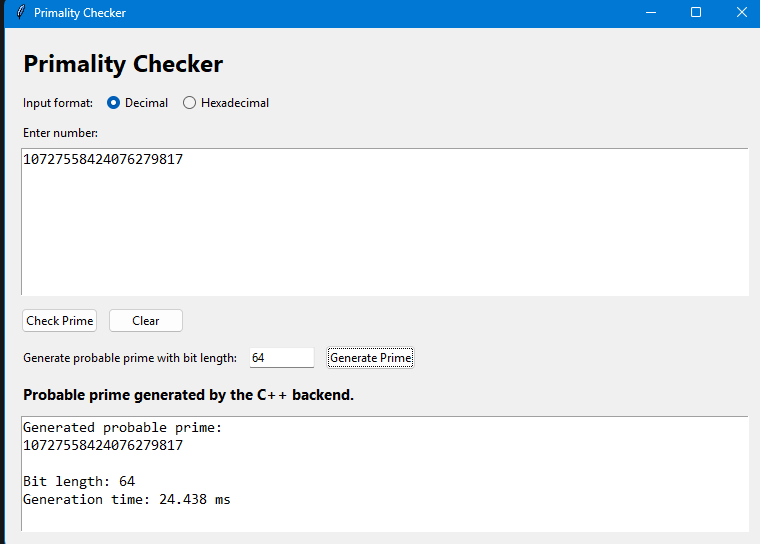
\includegraphics[width=0.92\textwidth,height=0.68\textheight,keepaspectratio]{gui_pictures/gui_generate_image.png}
        
        \vspace{0.15cm}
        {\footnotesize Prime-generation workflow for user-selected bit lengths.}
    \end{columns}
\end{frame}
% ----------------------------------------------------------------------
\section{6. Empirical Benchmarks and Practical Inferences}
% ----------------------------------------------------------------------
\begin{frame}{Observing Theory Vs Reality: The AKS Explosion}
    The goal of benchmarking is to observe the difference between deterministic polynomial bounds, and actual constant-factor engineering realities.
    
    \begin{figure}
        \centering
        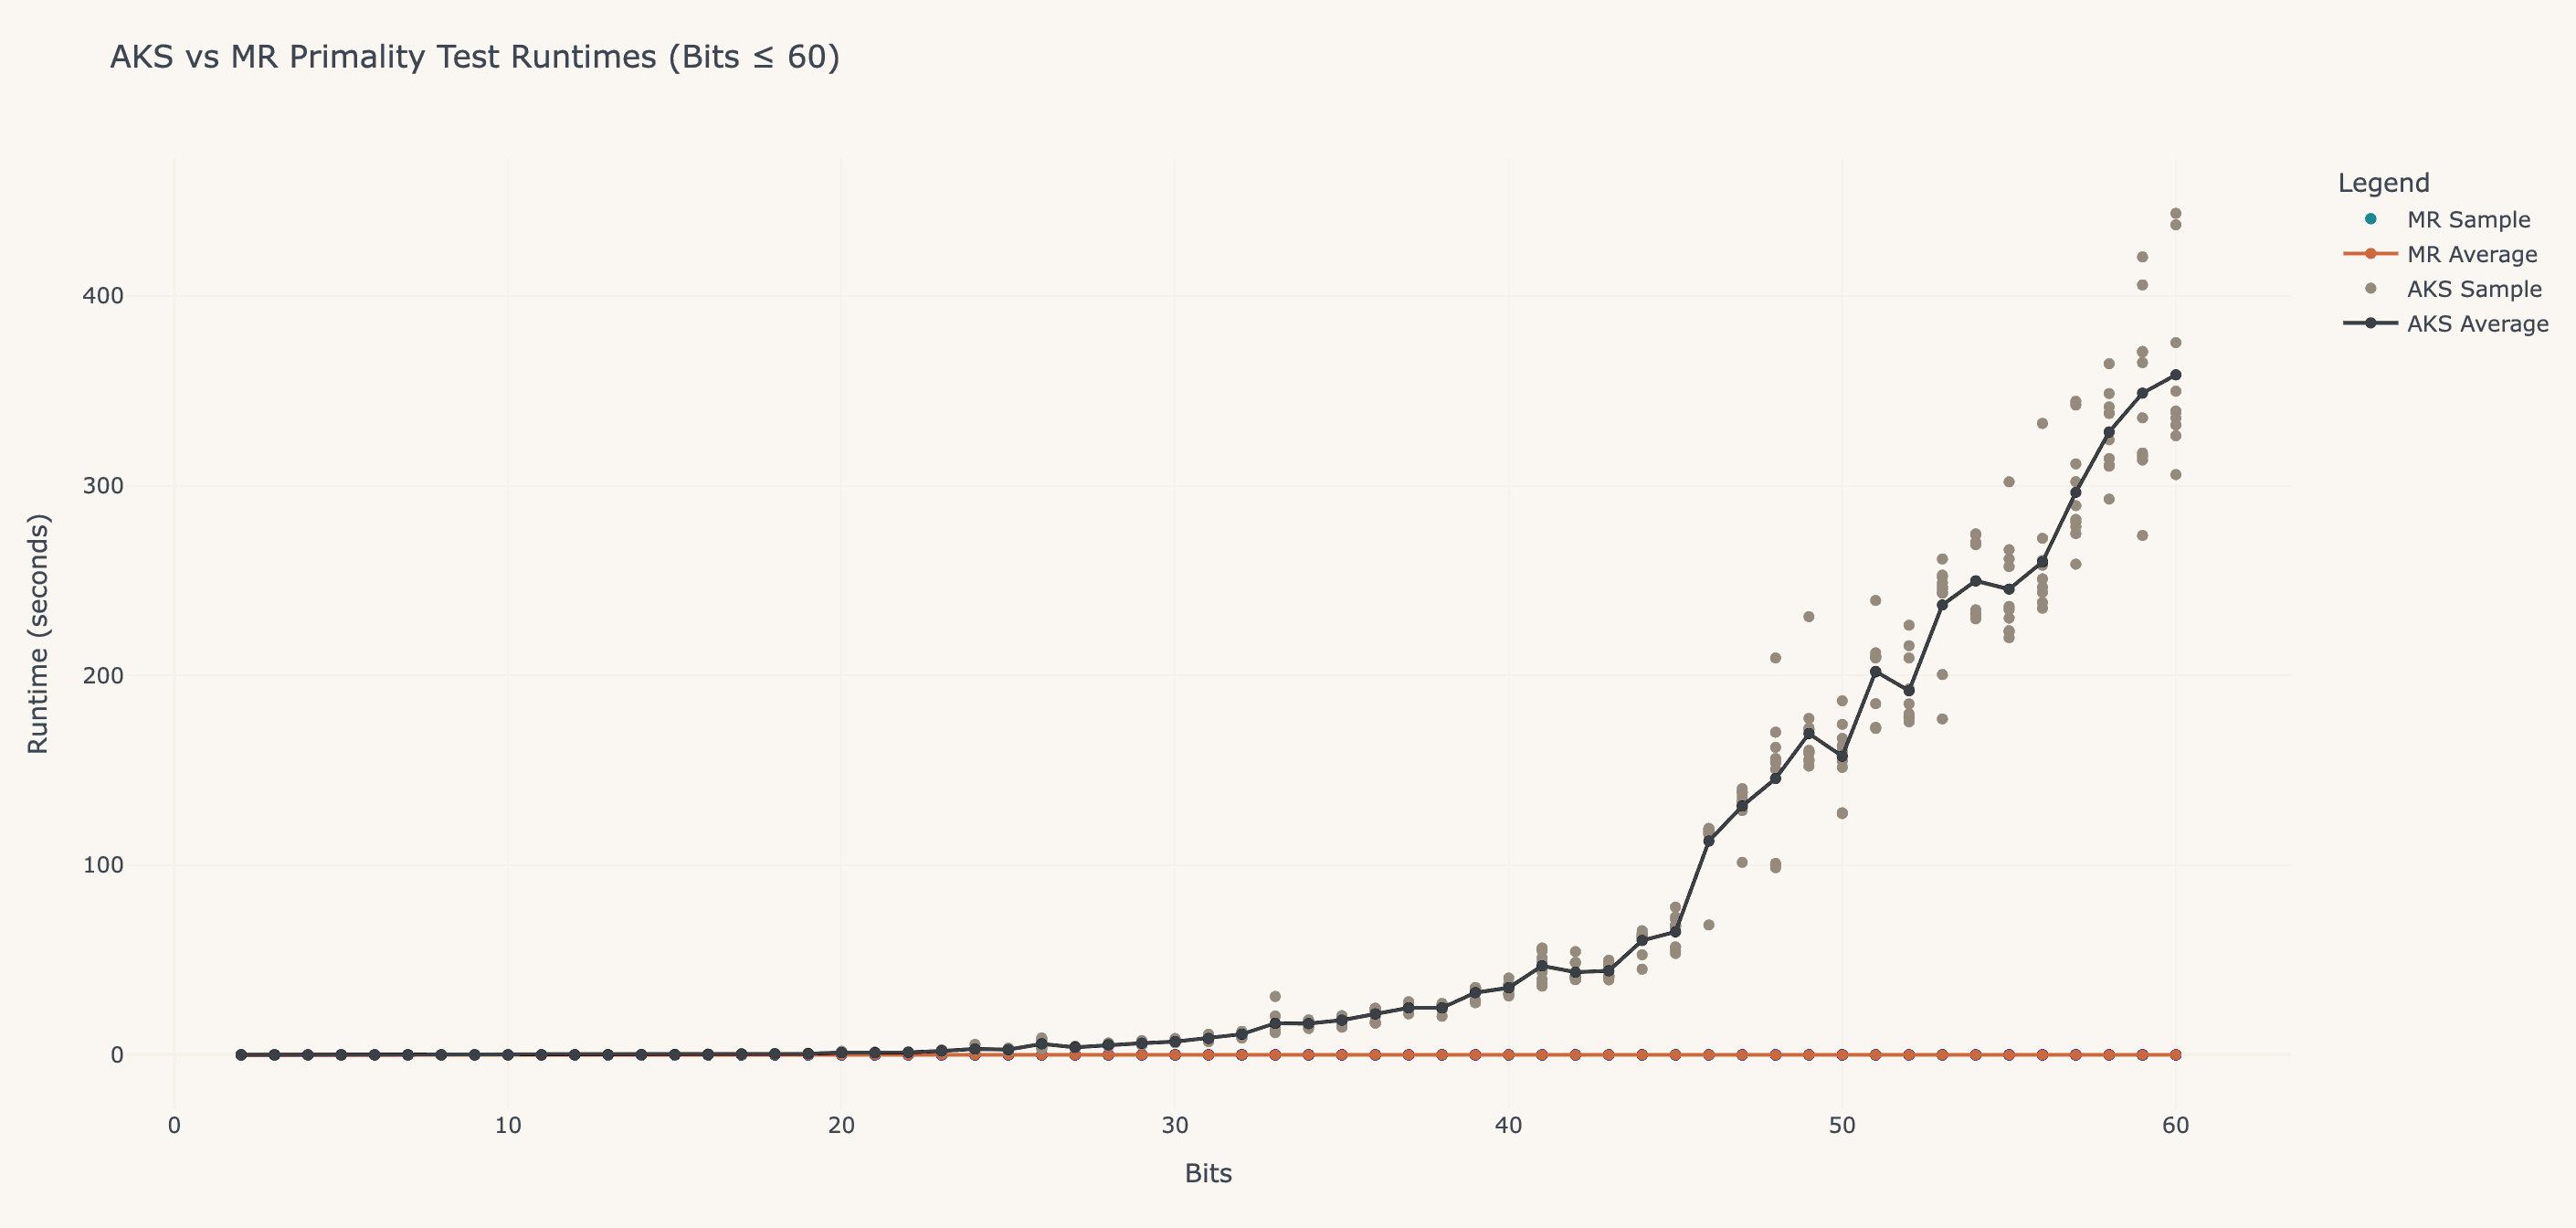
\includegraphics[width=0.7\textwidth]{images/aks_vs_miller_rabin_plot.png}
    \end{figure}
    
    \textbf{Practical Inference:} While AKS is guaranteed polynomial $\mathcal{O}(\log^{6} n)$, the graphical evidence shows a geometric wall. Testing a simple 60-bit prime severely delayed execution.
\end{frame}
\begin{frame}{Observing Theory Vs Reality: Miller-Rabin Dominance}
    \begin{figure}
        \centering
        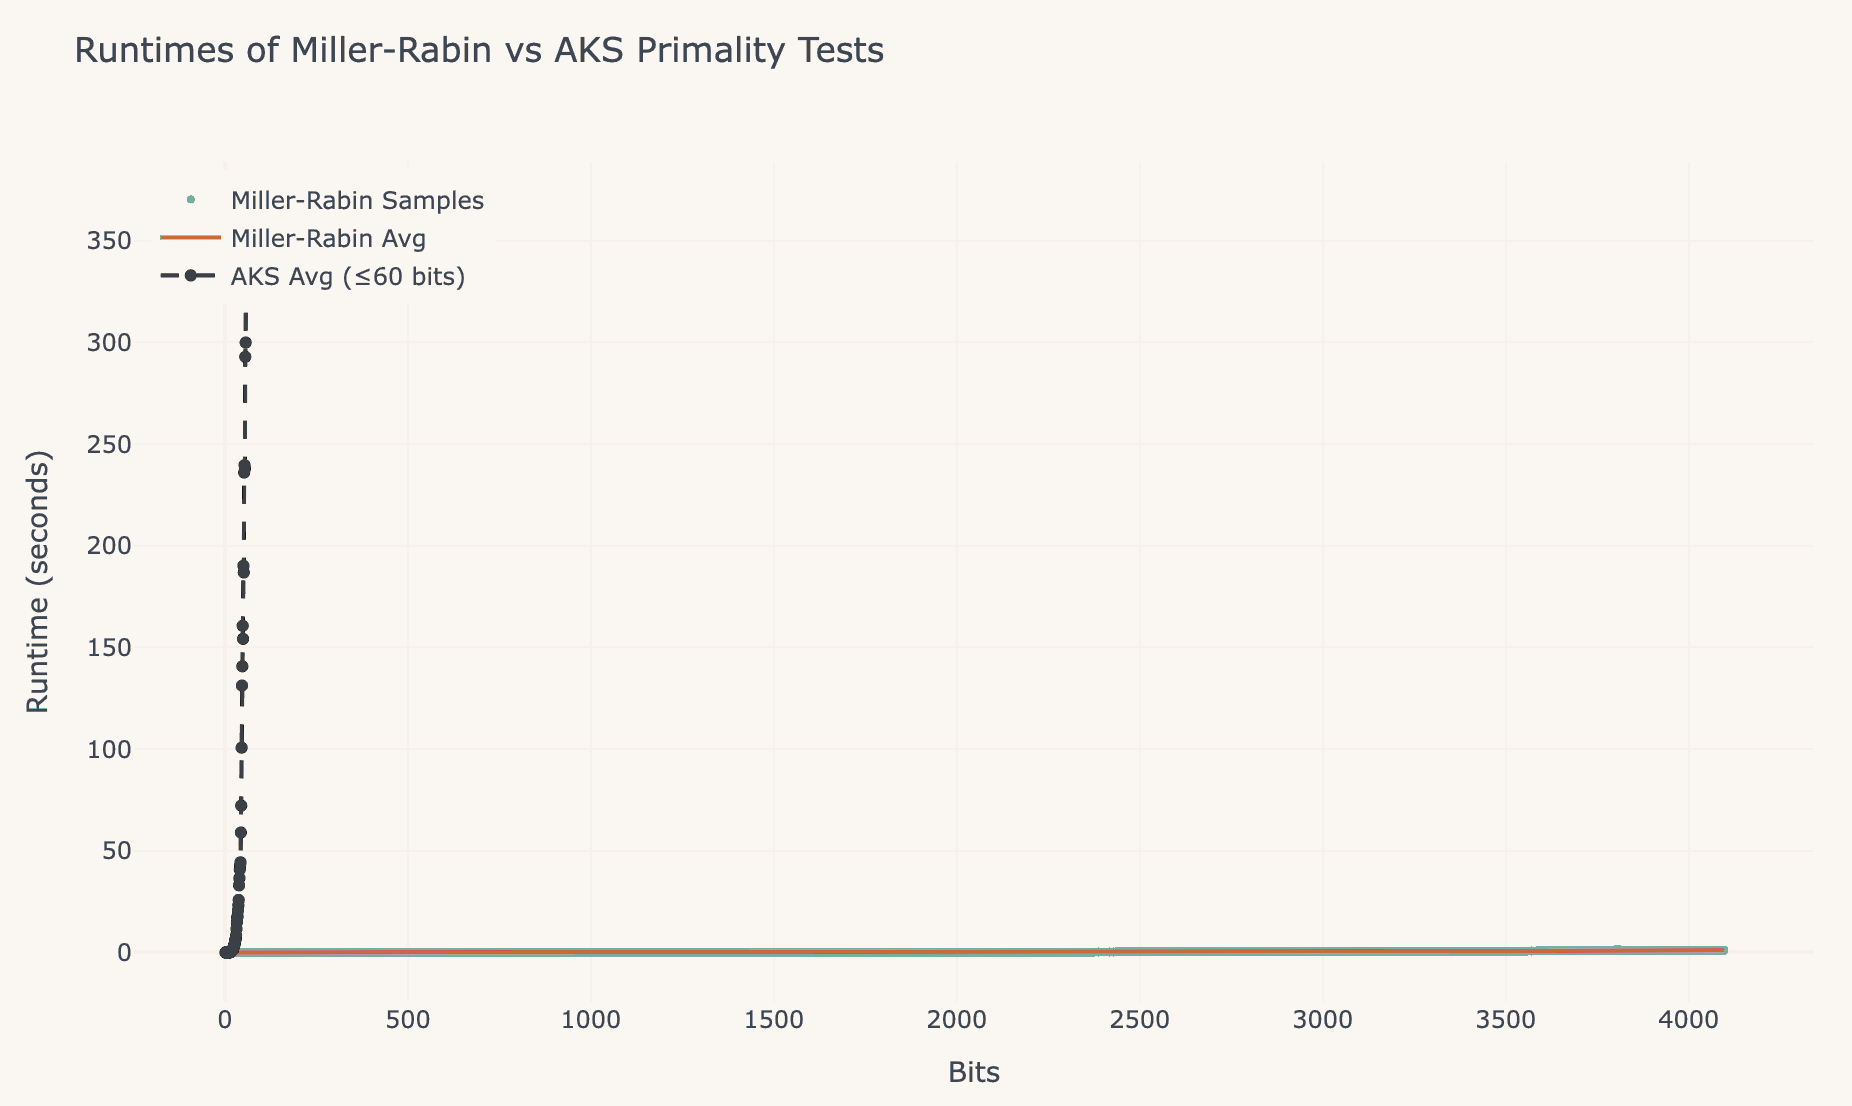
\includegraphics[width=0.8\textwidth]{images/aks_vs_miller_rabin_extended_plot.png}
    \end{figure}
    
    \textbf{Practical Inference:} Unlike AKS, Miller-Rabin operates on numbers in the thousands of bits while maintaining an execution profile almost visually flat against the base axis. For cryptographic needs (4096 bits), probabilistic testing is mandatory.
\end{frame}
\begin{frame}{Log-Scale Runtime Distribution}
    Comparing Prime Searching algorithms across aggregated datasets:
    \begin{figure}
        \centering
        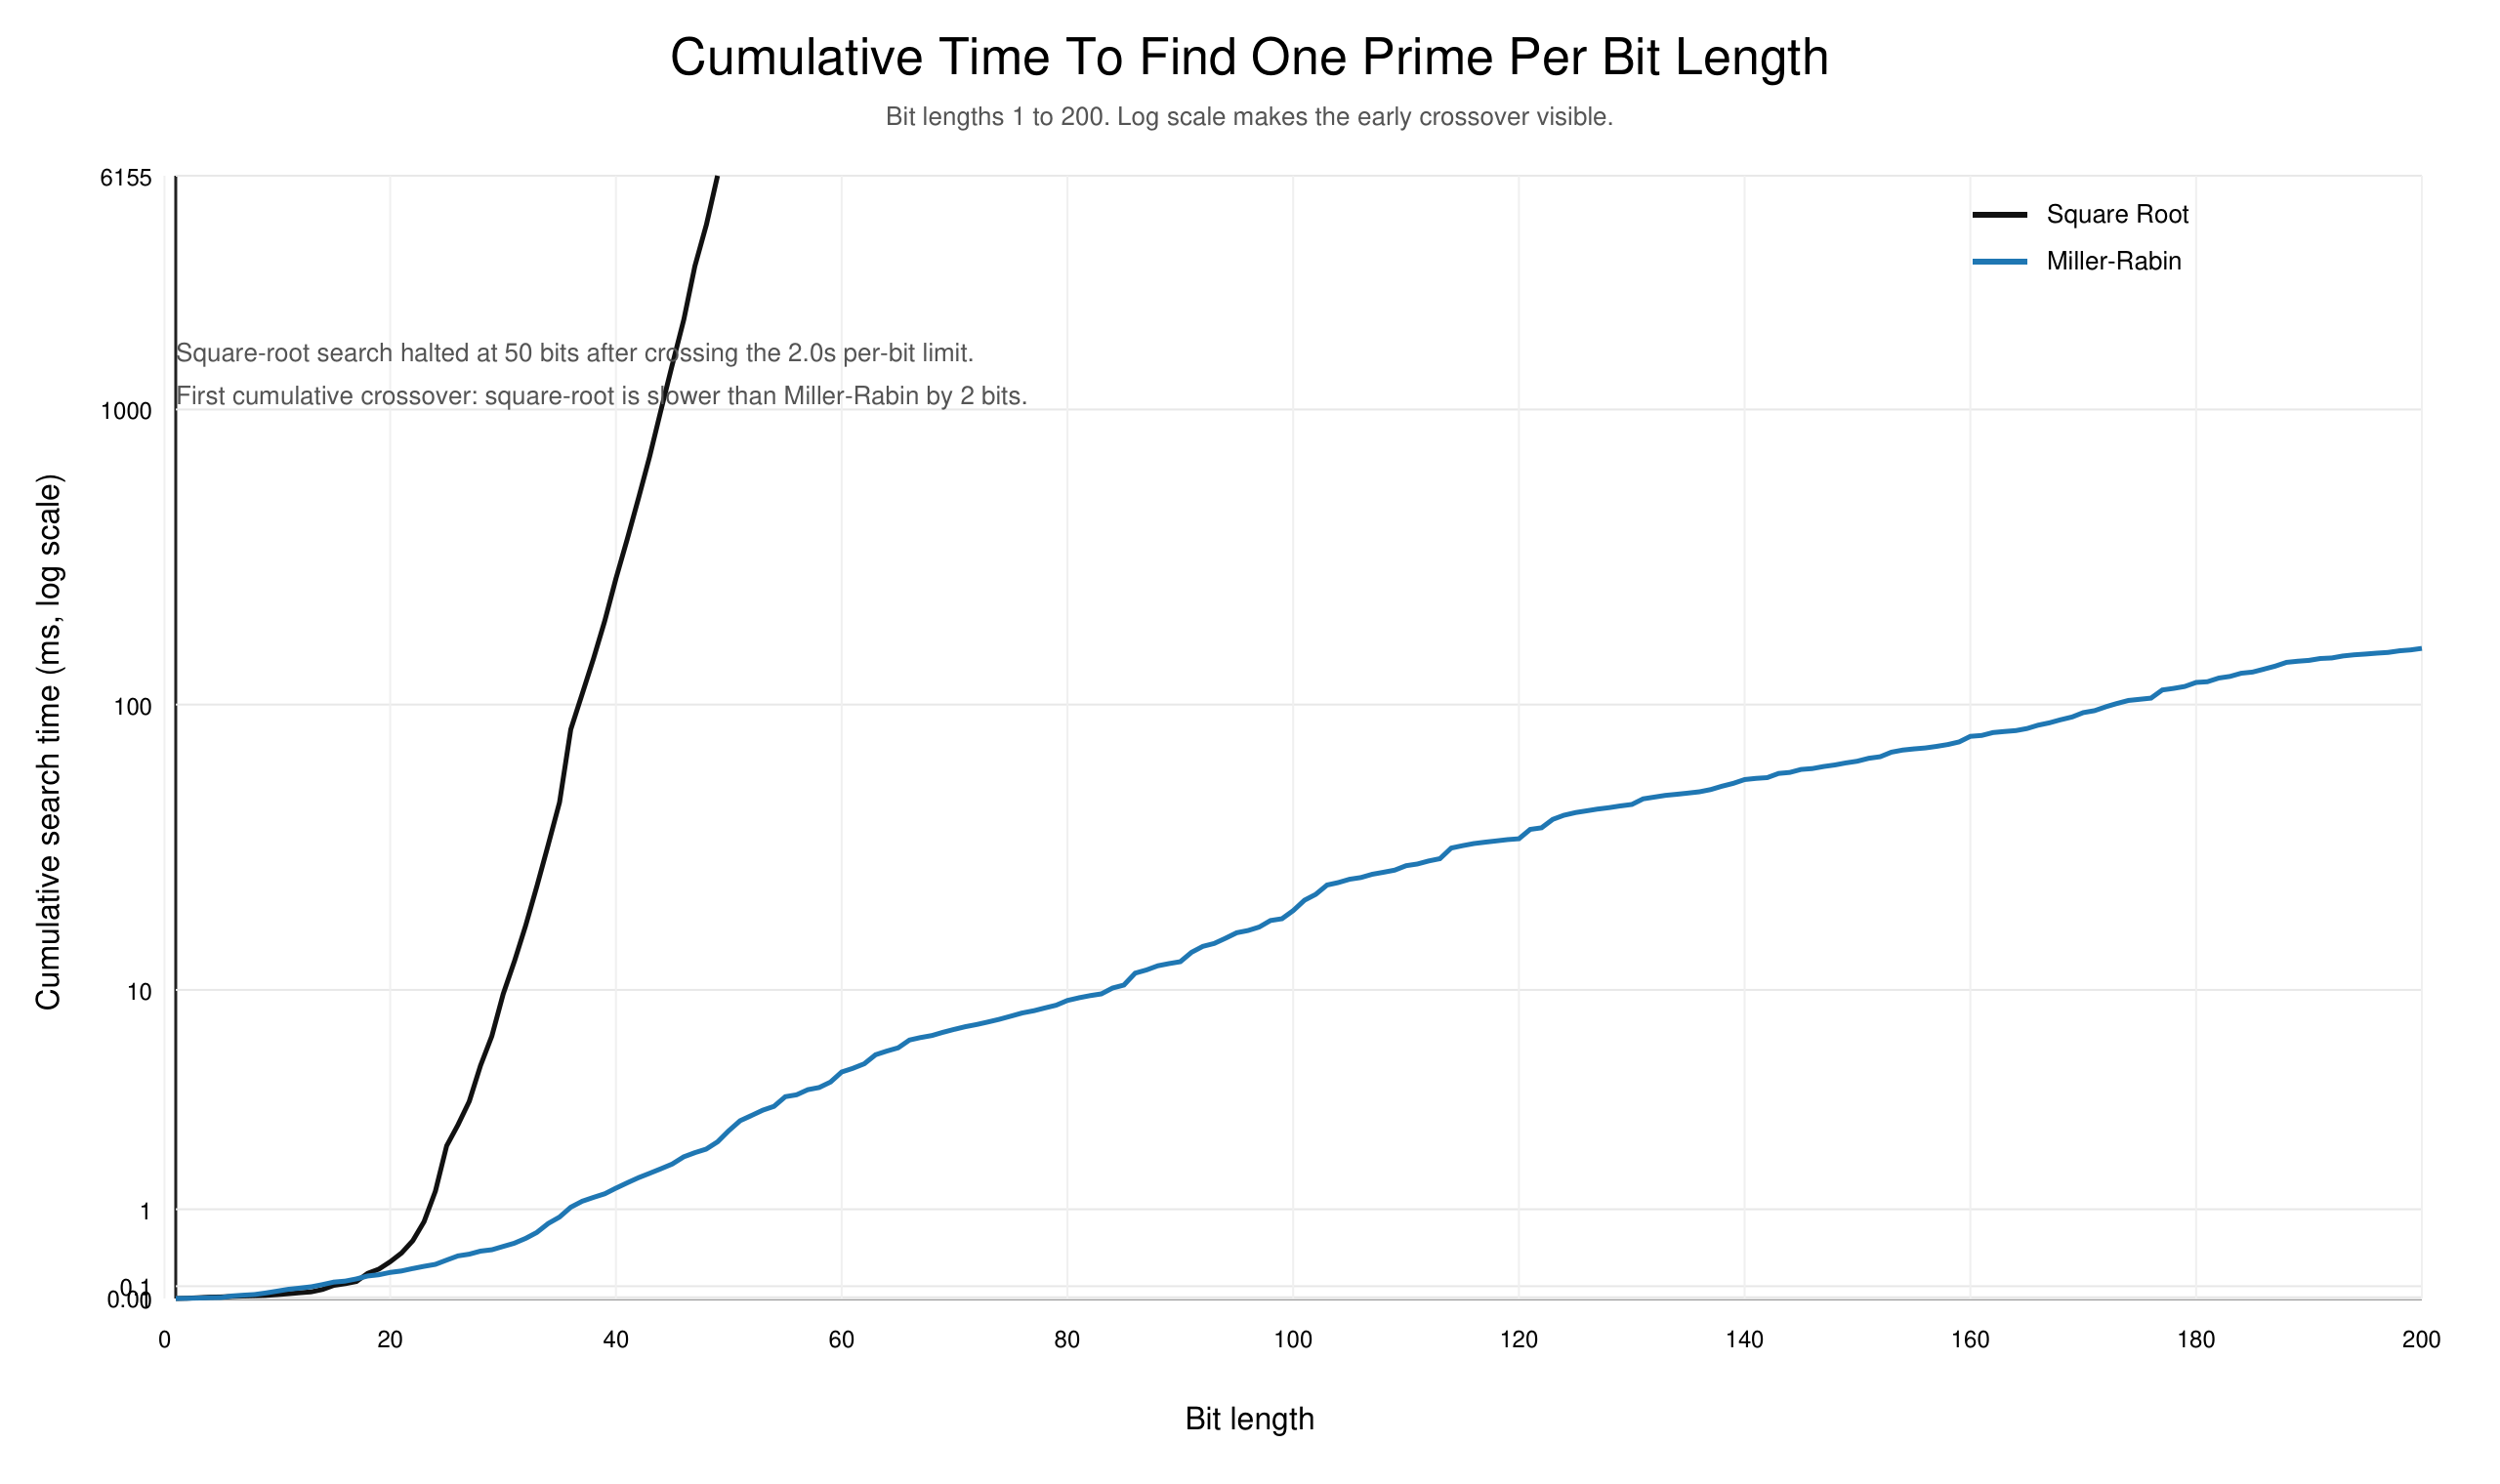
\includegraphics[width=0.85\textwidth]{images/bit_length_prime_search_comparison_log.png}
    \end{figure}
    
    \textbf{Practical Inference:} The Square-root baseline hits a computational limit instantly by 50 bits. Miller-Rabin is strictly required for driving sweeping prime-search boundaries efficiently.
\end{frame}
\begin{frame}{Engineering Isolation: Miller-Rabin Refinement}
    Even within a specific algorithm, custom engineering paths dictate performance.
    \begin{figure}
        \centering
        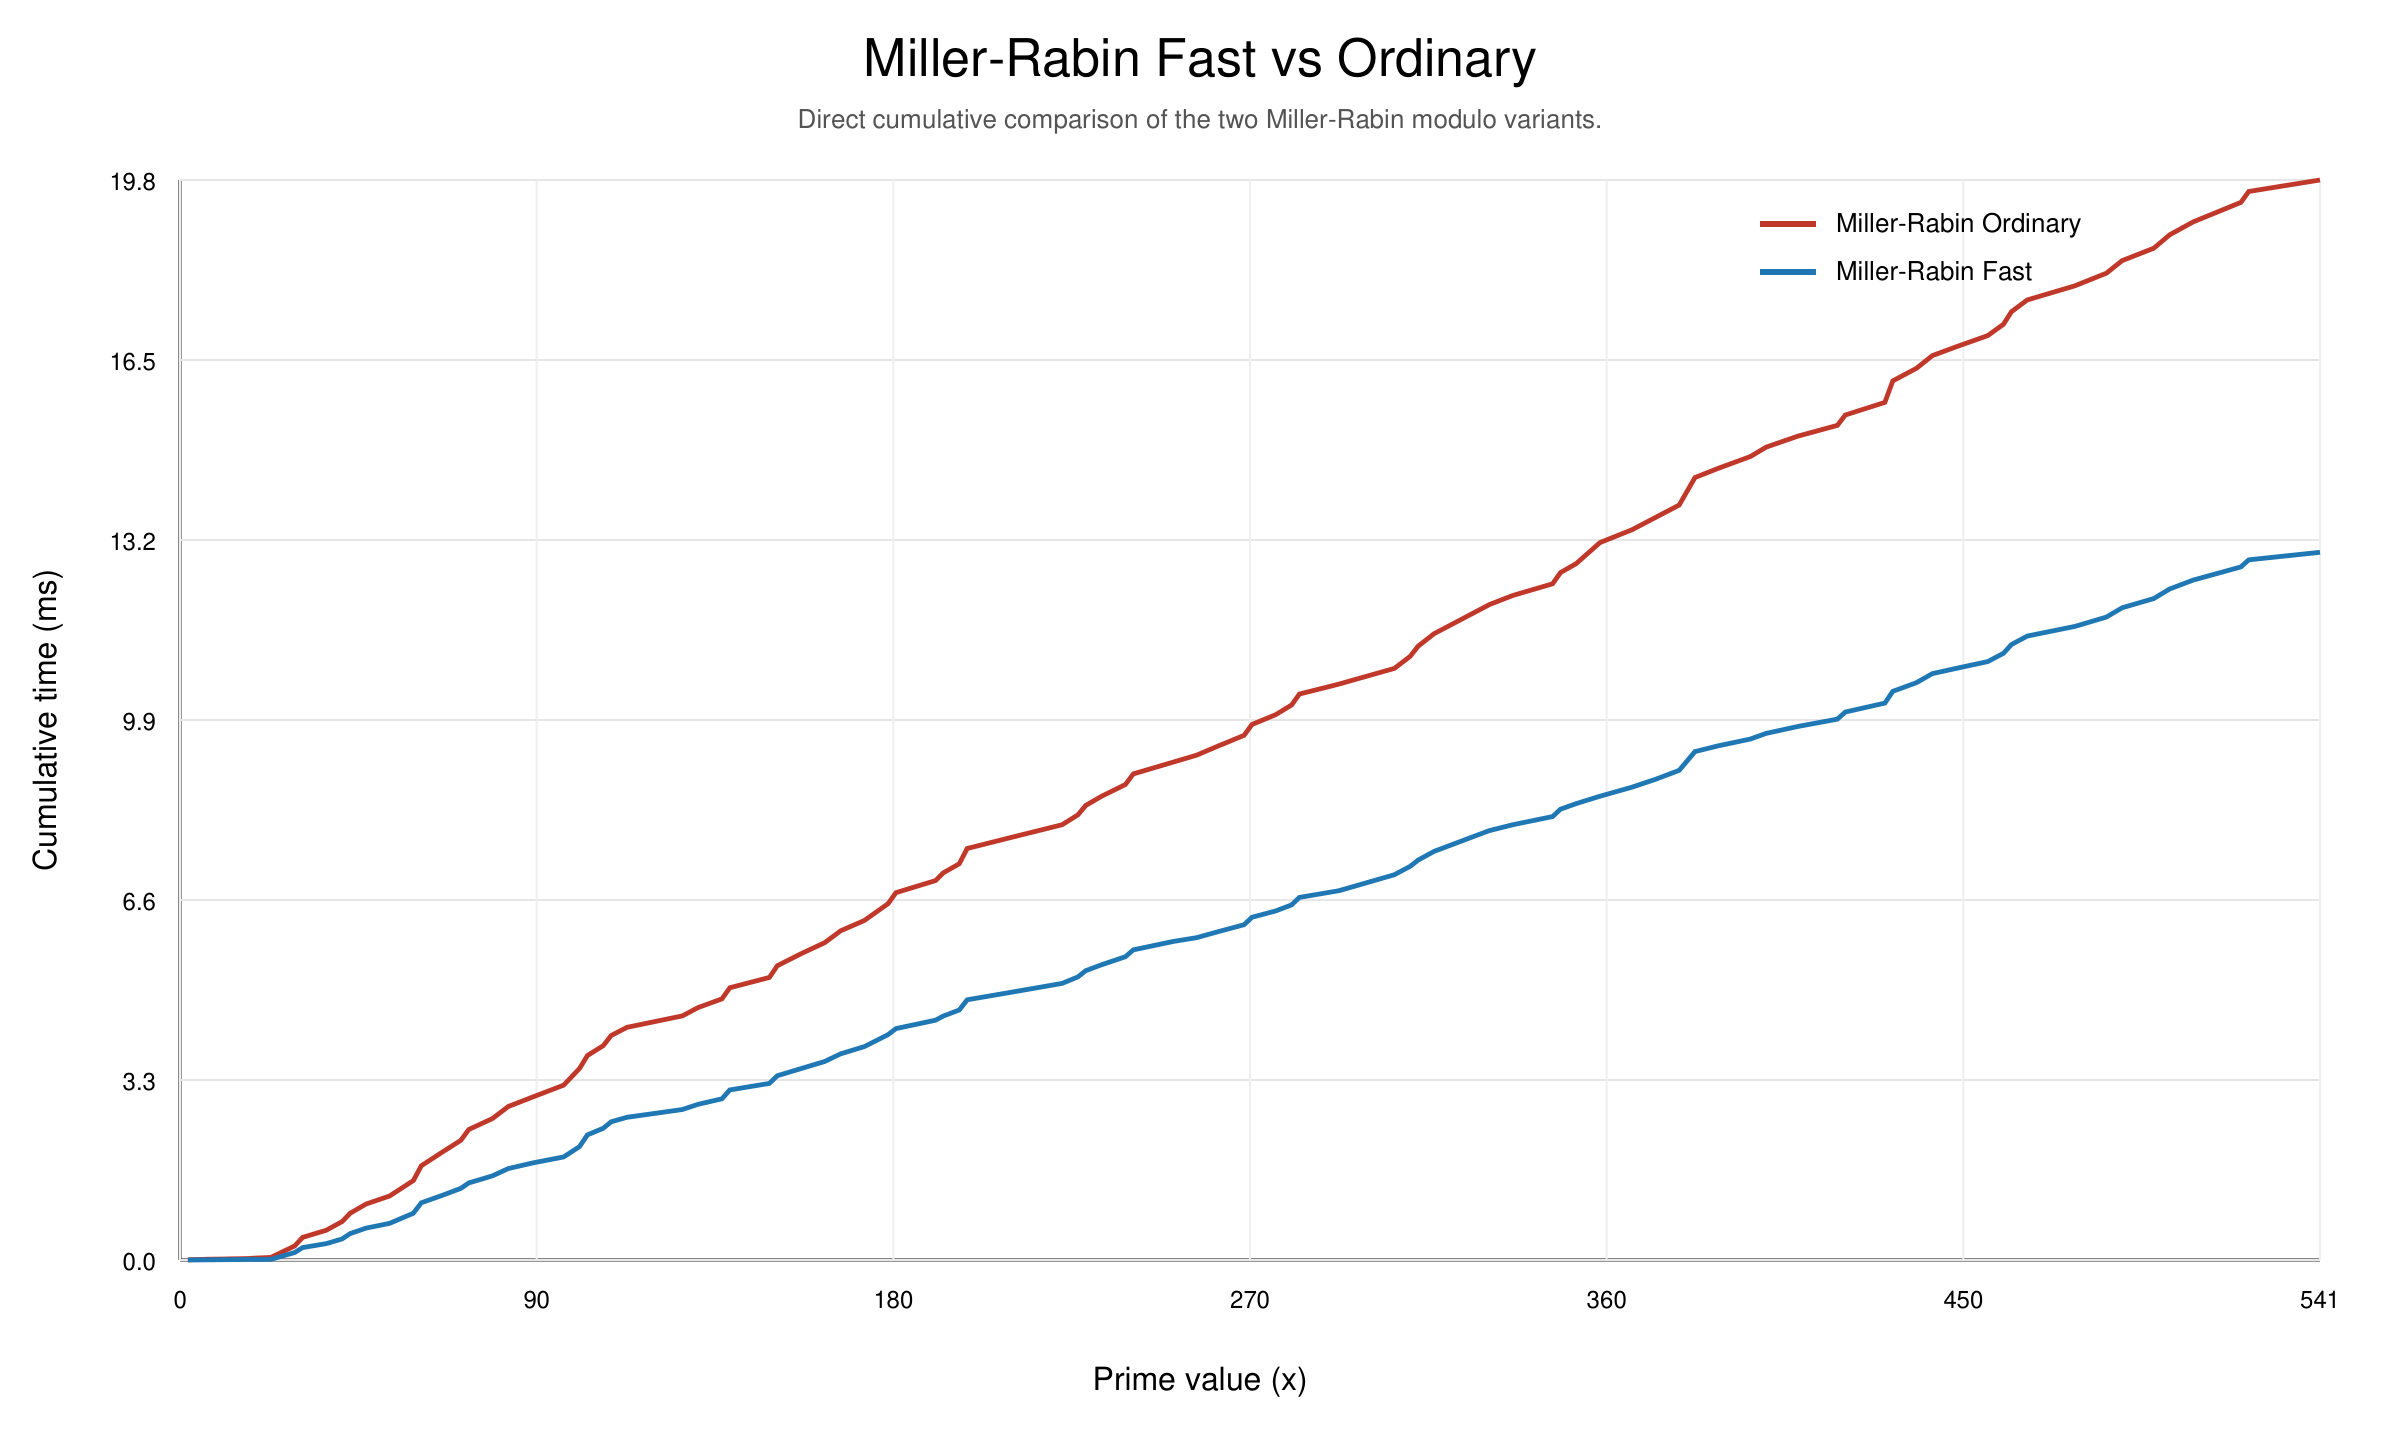
\includegraphics[width=0.85\textwidth]{images/miller_rabin_fast_vs_ordinary.png}
    \end{figure}
    
    \textbf{Practical Inference:} Comparing standard modular divisions against our custom \texttt{fast\_mod} engine highlights how critical low-level register isolation is. It saves vital overhead stacked exponentially across $k$-loops.
\end{frame}
% ----------------------------------------------------------------------
\section{7. Conclusion}
% ----------------------------------------------------------------------
\begin{frame}{Conclusion}
    \begin{itemize}
        \item<1-> \textbf{Mathematical Rigor:} We have observed step-by-step why the Miller-Rabin sequence rejects Carmichael combinations dynamically using field constraints.
        \item<2-> \textbf{Theoretical Limits:} We use the standard result that for odd composite $n$, at most $\frac{\varphi(n)}{4}$ bases can be strong liars.
        \item<3-> \textbf{Engineering Application:} Our custom `big\_int` and optimization filters bridged the gap between pure math and functional CPU execution cycles.
        \item<4-> \textbf{Final Takeaway:} A test that is "probabilistically true" executed in 150ms beats a test that is "deterministically true" but takes centuries. Engineering embraces manageable risk to unlock scale.
    \end{itemize}
    
    \onslide<5->
    \vspace{1cm}
    \centering
    \Large \textbf{Thank You.}
\end{frame}
\begin{frame}{Selected References}
    \begin{itemize}
        \item M. Agrawal, N. Kayal, and N. Saxena, \textit{PRIMES is in P}, Annals of Mathematics, 160(2), 781--793, 2004.
        \item G. L. Miller, \textit{Riemann's Hypothesis and Tests for Primality}, Journal of Computer and System Sciences, 1976.
        \item M. O. Rabin, \textit{Probabilistic Algorithm for Testing Primality}, Journal of Number Theory, 1980.
        \item OpenAI, \textit{ChatGPT}, used to write the AKS code implementation for this project, accessed April 5, 2026.
    \end{itemize}
\end{frame}
\end{document}
